\chapter{Literrature review} 
\label{Chapter2} 
\lhead{Chapter 2.\emph{Literrature review}}

This second chapter studies research done around WebSockets. The first
section is about the implementation of WebSockets server, the second is about
scalability. \\

\section{Implementation}

As in any project, in order to avoid future technical problems, it is better to
first study similar projects. The goal of this implementation study is to find a
suitable language and possibly a good library to run the experiment.

\subsection{WebSocket server implementation}

In order to narrow the library study, first a language needs to be selected.

\textbf{Language Selection}

Choosing a language for a project is often a compromise between the programmer
development background and the necessity of the application. Furthermore,
WebSocket servers can be developped in almost any languages.\\

This subsection does not aim at giving a comprehensive comparaison of all
existing WebSocket friendly languages. Node.js seems to be the perfect
environment for this study, therefore other languages will deliberatly be left
apart and the focus will be on explaining why Node.js is appropriate.\\

Node.js was specially invented to create real-time websites with push
capabilities \citep{Reference35}. Most languages run parallel tasks by using
threads but threads are memory expensive. Node.js is fundamentally different,
it runs as a single non-blocking and event-driven loop by using asynchronous
call back loops \citep{Reference37}. For this reasons, compared to other
languages, Node.js performs significantly better in highly concurrent
environment.\\

Node.js has many real-time engines. The next step is to carefully make a choice
between ws, Socket.io and Engine.io.\\  

\textbf{WebSocket implementation selection}

Deniz Ozger article's for medium.com \citep{Reference36} is a comprehensive study
of node.js real-time engines.\\

Ws is a pure WebSocket implementation, therefore it is interesting for testing
purpose but seldom used in real life projects.  The main drawback is the
communication may not work in case the browser does not support WebSockets.\\

Socket.io has some appreciable features namely it's connection procedure. First
it tries to connect to a server via WebSocket, in case it fails it downgrades
until it founds a suitable protocol. Moreover it tries to reconnect sockets
when connections fail.\\ 

Engine.io is a lower library of Socket.io. The connection procedure is the
opposite to Socket.io though. It first establishes a long polling connection
and only later tries to upgrade it to a better transport protocol. Therefore it
is more reliable because it establishes less connection.\\

In conclusion, Node.js and its real-time library engine.io seems a good choice
for our experiment. However better perfomance could be reached using an
heterogeneous implementation.


\subsection{Heterogeneous implementation with OpenCL}

As suggest John Stone paper's title \texttt{OpenCL: A parallel programming standard
for heterogeneous computing systems} \citep{Reference5} OpenCL is unanimously
considered as the refetence for heterogenous computing.\\

Historically, the first technology to take advantage of the massive parallel
nature of GPUs was Open Graphic Library (OpenGL). OpenGL is an application
programming interface (API) for rendering 2D and 3D vector graphics. Through
the insertion of little pieces of C-like codes in shader, developpers soon
realized graphic processing units (GPUs) could also be used for general
programming. This became known as General Purpose computation on GPUs (GPGPU)
\citep{Reference5}.\\

However, shadders can only be modified so much. As the need for more complex
applications arose Apple proposed the Khronos Group to develop a more general
framework: OpenCL. OpenCL is a low-level API accelerating applications with
task-parallel or data-parallel computations in a heterogeneous computing
environment. Indeed OpenCL not only allows the usage of CPUs but also any
processing devices like GPUs, DSPs, accelerators and so on \citep{Reference5}.
If generally on desktop the diversity of processing devices is quite low, it is
the opposite for mobile. Embedded systems for real-time multimedia journal
published a paper \citep{Reference3} highlining the advantages of using OpenCl
in mobile browser.\\

OpenCL doesn't guarantee a particular kernel will achieve peak performance on
different architectures. The nature of the underlying hardware may induce
different programming strategies. Multi-core CPU architecture is definitely the
more popular. But the recent specification published by Khronos to take GPU
computing to the web is bound to raise programmers interest toward GPUs
architecture \citep{Reference30}.\\ 

\textbf{CPUs architecture}

Modern CPUs are typically composed of a few high-frequency processor cores.
CPUs perform well for a wide variety of applications, but they are optimal for
latency sensitive workloads with minimal parallelism. However, to increase
performance during arithmetic and multimedia workloads,  many CPUs also
incorporate small scale use of single instruction multiple data (SIMD).\\

\textbf{GPUs architecture}

Contemporary GPUs are composed of hundreds of processing units running at low
frequency. \\

As a result GPUs are able to execute tens of thousands of threads. It is this
ability which makes them so much more effective then CPUs in a highly parallel
environment. Some research even claim a speedup in the order of 200x over
JavaScript. \citep{Reference3}\\

The GPU processing units are typically organized in SIMD clusters controlled by
single instruction decoders, with shared access to fast on-chip caches and
shared memories. Massively parallel arithmetic-heavy hardware design enables
GPUs to achieve single-precision floating point arithmetic rates approaching 2
trillions of instructions per second (TFLOPS). \citep{Reference5}\\

Although GPUs are powerful computing devices, currently they still often
require to be managemed by a host CPU. Fortunately OpenCL is designed to be used in
heterogeneous environment. It abstracts CPUs and GPUs as “compute devices”.
This way, applications can query device attributes to determine the
properties of the available compute units and memory systems.
\citep{Reference5}\\

All the same, even if OpenCL's API hides the hardest part of parallel
programming a good understanding of the underlying memory model leads to more
efficient codding. Along with general advises on how to build an OpenCL
cluster, details about the memory model are given in the following paper:
\citep{Reference4}.\\

\textbf{Platform model}

CPU and GPU are called “compute devices”. A single host regroups one or more
compute devices and has its own memory. Each compute device is composed of one
or more cores also called “compute units”. Each compute unit has its own memory
and is divided into one or more SIMD threads or “processing elements” with its
own memory. \citep{Reference4}\\

\begin{figure}[H] \centering
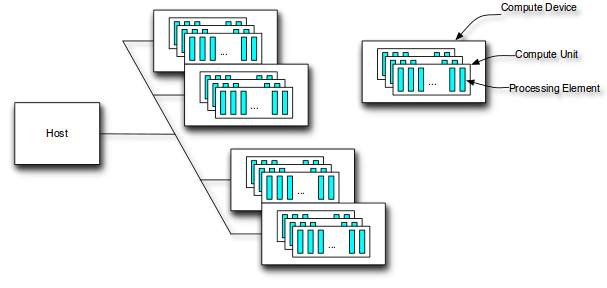
\includegraphics[width=\textwidth]{./Figures/plateform_model.png}
\caption[Plateform model]{Plateform model \citep{Reference4}}
\label{fig:plateform_model} \end{figure}


\textbf{Memory model}

OpenCL defines 4 types of memory spaces within a compute device. A large
high-latency “global” memory corresponding to the device RAM. This is a none
cached memory  where the data is stored and is available to all items. A small
low-latency read-only “constant” memory which is cached. A shared “local”
memory accessible from multiple processing elements within the same compute
unit and a “private” memory accessible within each processing element. This
last type of memory is very fast and is the register of the items
\citep{Reference4}.\\

\begin{figure}[H] \centering
  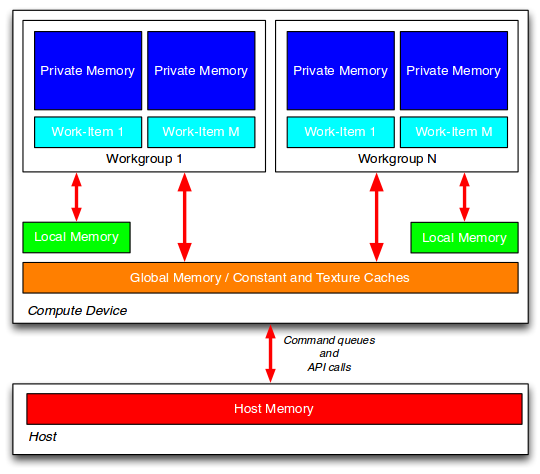
\includegraphics[width=0.6\textwidth]{./Figures/memory_model.png}
  \caption[Memory model]{Memory model \citep{Reference4}}
  \label{fig:memory_model} 
\end{figure}

In conclusion, OpenCL provides a fairly easy way to write parallel code but to
reach an optimal performance / memory access trade off programmers must choose
carefully in where to save their variables in memory space.\\

\textbf{Global and local IDs}

Finally, at an even lower level, work-items are scheduled in work–groups.
This is the smallest unit of parallelism on a device. Individual work-items in
a work–group  start together at the same program address, but they have their
own address counter and register state and are therefore free to branch and
execute independently \citep{Reference4}.\\

\begin{figure}[H] \centering
  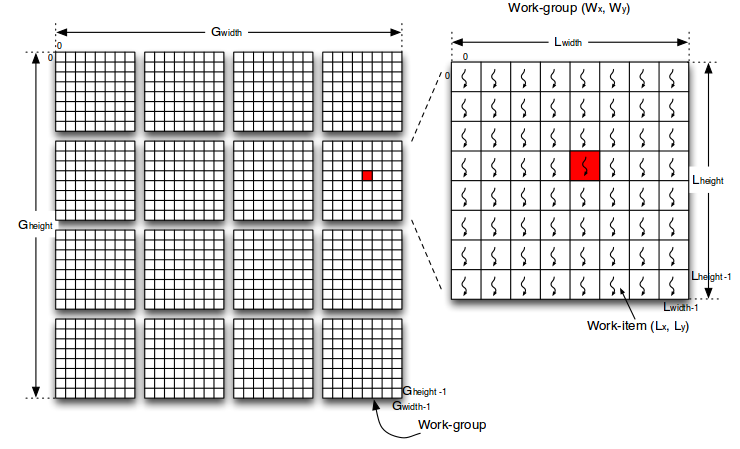
\includegraphics[width=\textwidth]{./Figures/id.png} 
  \caption[Work - group]{Work Group \citep{Reference4}} 
  \label{fig:id} 
\end{figure}


On a CPU, operating systems often swap two threads on and off execution
channels. Threads (cores ) are generally heavyweight entities and those context
switches are therefore expensive. By comparison, threads on a GPU ( work-items
) are extremely lightweight entities. Furthermore in GPUs, registers are
allocated to active threads only. Once threads are complete, its resources are
de-allocated.  Thus no swapping of registers or state occurs between GPU
threads. \citep{Reference4}\\

As can be deduced from this section about the underlying memory model, OpenCL is a
fairly low-level API. In fact, the programming language used is a derivate of
the C language based on C99. A language web developers will most likely be
unfamiliar with. Khronos anticipated this and developed the web computing
language (WebCL).\\

\subsection{WebCL}

WebGL and WebCL are JavaScript APIs over OpenGL and OpenCL's API. This allows
web developers to create application in an environment they are used to.\\

In the first place, OpenCL was developed because of web browser's increasing
need for more computational power. A necessity which arose from heavy 3D
graphics applications such as on-line games and augmented reality. However,
OpenCL doesn’t provide any rendering capability, it only processes huge amounts
of data. That is why OpenCL was designed for inter-operation with OpenGL.
WebCL/WebGL interoperability builds on that available for OpenCL/OpenGL. WebCL
provides an API for safely sharing buffers with OpenCL. This buffer is inside
the GPU which avoids the back and forth copy of data when switching between
OpenGL and OpenCL processes. Further precision about the interoperability are
discussed in this paper: \citep{Reference6}.\\

GPU computing is quite a new notion. But it is a fast evolving field of
research. Single GPUs are not enough anymore, the trend is moving towards GPU
clusters.\\

\subsection{GPU clusters}

Most OpenCL applications can utilize only devices of the hosting computer. In
order to run an application on a cluster, the program needs to be split to take
advantage of all devices. Virtual OpenCL (VirtualCL) is a wrapper for OpenCL.
It provides a platform where all the cluster devices are seen as if located on
the same hosting node. Basically, the user starts the application on the master
node then VirtualCL transparently runs the kernels of the application on the
worker nodes. Applications written with VirtualCL don't only benefit from the
reduced programming complexity of a single computer, but also from the
availability of shared memory and lower granularity parallelism. Mosix white
paper \citep{Reference7} explains more in depth the VCL's functionement.
\\

OpenCL and VirtualCL are powerful tool to create highly parallel clusters.  But
current implementation with CPUs only already reach a million concurrent
connections \citep{Reference13}. So far there is simply no need for more
powerful clusters.

However, all company don't have acccess to dual Quad-core Xeon CPUs used in
Kaazing cluster to reach a million concurrent connections. Usual practice is to
build a scalable cluster, to ajust computing power in fonction of the needs.

\section{Scalability}

The growth of distributed computing has changed the way web application are
designed and implemented. If compared with today standards, applications used
to be deployed so as to say at prototype stage. That is, they were designed to
work on a fixed number of servers and not able to ajust as the userbase grows.
As the number of connections increases, the load on the servers rises and thus
the latency grows. Ideally, an application should aim at a stabil latency,
otherwise the application can missbehave.\\ 

On the server side, the nodes will begin to be overloaded and struggle to
service the client with reasonable response time.\\ 

Also, if the servers are overwhelmed they buffer the responses to the clients
and then catch up later on . As a result, the clients can be flooded when the
load goes down. The sudden rush of message can provoke an unexpected behavior
from the servers and can even lead to disconnections.\\

Nowadays, designing an application without scalability and load balancing in
mind is unimaginable. Historically, the reaction to an overloaded server
has always been to scale up.\\

\subsection{Scaling up}

Scaling up or vertically basically means upgrading the infrastructure.
Depending on the needs of the application, the processor, the memory, the
storage or the network connectivity can be improved.\\

Further performance can be gained by dividing tasks. It only requires to
identify the services  running idependantly or the using message based
communication. Those could then be relocated on different nodes.\\

The main advantage of scaling vertically is it does not involve any software
changes and little infrastructure changes. Therefore it is an easy way to
increase performances. However for large application, scaling up might prove
impossible or at least not economicaly profitable. In case the infrastrucure 
is already equiped with the lastest hardware generation, the tiniest
increase in performance will impact greatly the price. For example, a high
range processor offering ten pourcent more computation power is going to be
many times more expensive. Similarly, a memory upgrade could require remplacing
all current modules for higher density ones.\\

Moreover, scaling up neither answers availability nor uptime concerns. The
system is monolithic and has a single point of failure. Therefore contemporary
project usually scale out and use parallel computing.\\

\subsection{Scaling out}
				
Scaling out or horizontally, answers most of the problems unsolved by scaling
vertically. In a first approach lets ignore the software complexity.  Scaling
out offers almost unlimitted performance increase and at low cost! If the
application is designed to be spread out on multiple nodes, the performance of
an infrastructure can be doubled by simply using twice as much servers. Also it
is fairly easy to add some redundant server to insure uptime. Plus, compared to
scaling up, once the sofware is developped the costs are linear.\\

When scaling out, the infrastructure implementation is not as much a problem as
the code implementation. The expenses are shifted from hardware to developpment
costs.\\

\textbf{Code implementation}

Developping a parallel code is quite complicated and all applications can not
be parallized. In 1967 Gene M. Amdhal defined the so called Amdahl's law which
is still used today to define the maximum to expect when parallelizing a code
\citep{Reference10}. \\

Each software can be divided in two separete parts, the parallel part and the
sequential part. Parallel computing does not improve the sequential part. If a
the code is mainly sequential, then increasing the number of processors will
only cause the parallel part to finish first and stay idle waiting for the
sequential part to finish.\\ 

Assuming P is the portion of a program that can be parallelized and 1 - P  is
the portion that remains serial, then the maximum speedup that can be achieved
using N processors is: 

$$speedup(N) = \frac{1}{(1-P) + \frac{P}{N}} $$

If 70\% of the program can be run in parallel (P = 0.7) the maximum expected
speedup with 4 processors would be:

$$speedup(N) = \frac{1}{(1-0.7) + \frac{0.7}{N}}$$

$$speedup(4) = 2.1$$

When the number of processors reaches a certain point, the speed up will be:


$$\lim\limits_{N \to \infty} speedup(N)= \frac{1}{1-P} = 3.3$$\\


Nathan T. Hayes's paper for Sunfish Studio \citep{Reference8} studies how
parallel computing can profit the motion picture industrie. The following chart
present the maximum speedup which can be expected from an application in
function of the pourcentage of parallel code in the programme.\\

\begin{figure}[H] 
  \centering
  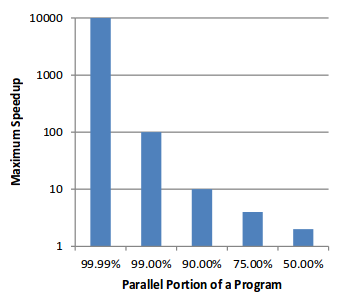
\includegraphics[width=0.5\textwidth]{./Figures/amdahl.png}
  \caption[Amdahl law]{Amdahl law \citep{Reference8}} 
  \label{fig:amdahl} 
\end{figure}

The figures speak for itslelf, to envisage parallel computing, the portion of
parallel code must be very high.

However, Amdahl's law is based on assumption which are hardly verified in
pratique. Following are sumed up reasons not to give to much importance to
Amdahl's law \citep{Reference34}:

\begin{itemize} 
  \item The number of thread is not always always equivalent to the number of processors.  
  \item The parallel portion does not have a perfect speedup. Computation power is used
    for communication between processus. Also some ressources like caches and bandwidth
    have to be shared across all the processors.  
  \item Allocating, delocating and switching threads introduce overhead, overhead growing
    linearly with the number of thread.  
  \item Even an optimized code will not have perfectly synchronised threads, at some point
    some processus will have to wait for others to finish.	
\end{itemize}


Amdahl's law has long been used as an argument against massively parallel
processing. In 1988 Gustafson law came as an alternative to Amdahl's law to
estimate the speedup. In both law, the sequential portion of the problem is
supposed to stay constant. But in Gustafson's law the overall problem size
grows proportionally to the number of cores. As a result, Gustafson's gives
slightly different results to Amdahl's and encourage the use of parallel
computing.\\

However later studies tends to contest the legimity of both laws. Yuan Shi's
paper \citep{Reference9} even proves both theory are but two different
interpretations of the same law. He concludes his study by saying these laws
are too minimalist and what computer scientist really need is a practical
engineering tool that can help the community to identify performance critical
factors.\\

\textbf{Infrastructure implementation}

Beside coding complication, scaling out also brings infrastructure changes.
A third party must be in command of all servers. This master server is also called
load balancer. Its role is to distribute the work evenly between the workers and thus
completly hides the complexity to the user.\\


